\documentclass[11pt, a4paper]{article}

\usepackage[utf8x]{inputenc}
\usepackage[left=1.8cm, text={18cm, 25cm}, top=2.2cm]{geometry}
\usepackage[T1]{fontenc}
\usepackage[czech]{babel}
\usepackage{xcolor}
\usepackage[colorlinks=true,linkcolor=black,urlcolor=black,bookmarksopen=true,unicode=true]{hyperref}
\usepackage{bookmark}
\usepackage{graphicx}

\graphicspath{{fig/}}

\title{
\includegraphics[width=0.4\linewidth]{logo_en.png}\vspace{1cm}\\\huge{Projekt IDS\\2020/2021}\\\vspace{1cm}4. a 5. část - poslední SQL skript, dokumentace}
\author{Adrián Kálazi, Kevin Lackó\\xkalaz00, xlacko08}
\date{}

\begin{document}

    \maketitle

    \bigskip

    \begin{center}
        \textbf{\Large{Zadanie IUS č. 49 - Bug Tracker}}
    \end{center}

    Vytvořte informační systém pro hlášení a správů chyb a zranitelností systému.
    Systém umožňuje uživatelům hlásit bugy, jejich závažnosti a moduly, ve kterých se vyskytly, ve formě tiketů.
    Tikety mohou obsahovat hlášení o více než jednom bugu a stejný bug může být zahlášen více uživateli.
    Bug může (ale nemusí) být zranitelností a v tomto případě zaevidujeme i potenciální míru nebezpečí zneužití této zranitelnosti.
    V případě zahlášení bugů, odešle systém upozornění programátorovi, který zodpovídá za daný modul, přičemž může odpovídat za více modulů.
    Programátor pak daný tiket zabere, přepne jeho stav na "V řešení" a začne pracovat na opravě ve formě Patche.
    Patch je charakterizován datem vydání a musí být schválen programátorem zodpovědným za modul, které mohou být v různých programovacích jazycích.
    Jeden Patch může řešit více bugů a současně řešit více tiketů a vztahuje se na několik modulů.
    Samotní uživatelé mohou rovněž tvořit patche.
    Takové patche však musí projít silnější kontrolou než jsou zavedeny do systému.
    Kromě data vytvoření patche rovněž evidujte datum zavedení patche do ostrého provozu.
    Každý uživatel a programátor je charakterizován základními informacemi (jméno, věk, apod.), ale současně i jazyky, kterými disponuje, apod.
    V případě opravení bugů, mohou být uživatele upozorněni na danou opravu a případně být odměněni peněžní hodnotou (podle závažnosti bugu či zranitelnosti).


    \newpage


    \section{Use case diagram}
    \label{sec:use-case-diagram}
    \begin{center}
        \vspace*{\fill}
        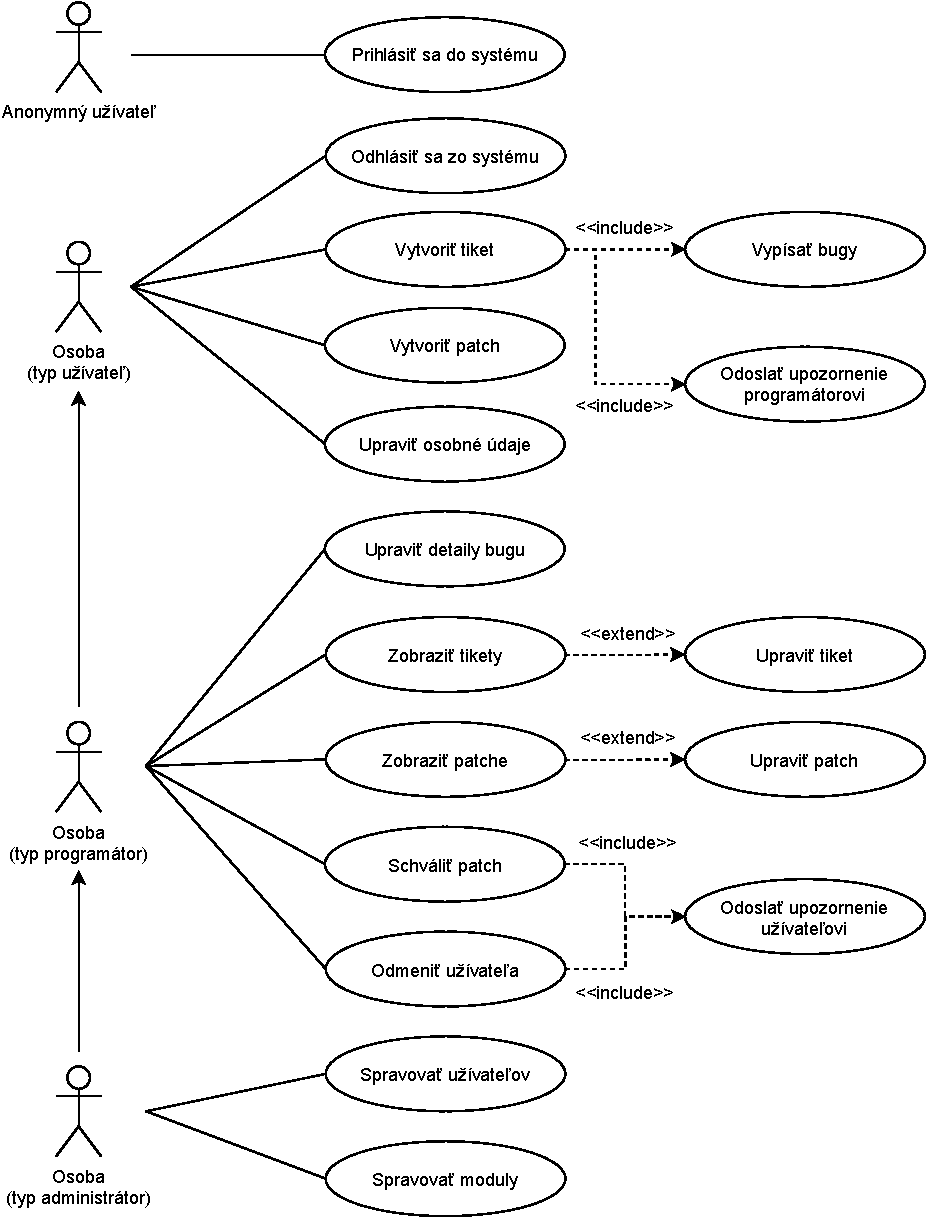
\includegraphics[width=0.9\linewidth]{UC_diagram.pdf}
        \vspace*{\fill}
    \end{center}

    \newpage


    \section{Entity relationship diagram}
    \label{sec:entity-relationship-diagram}
    \begin{center}
        \vspace*{\fill}
        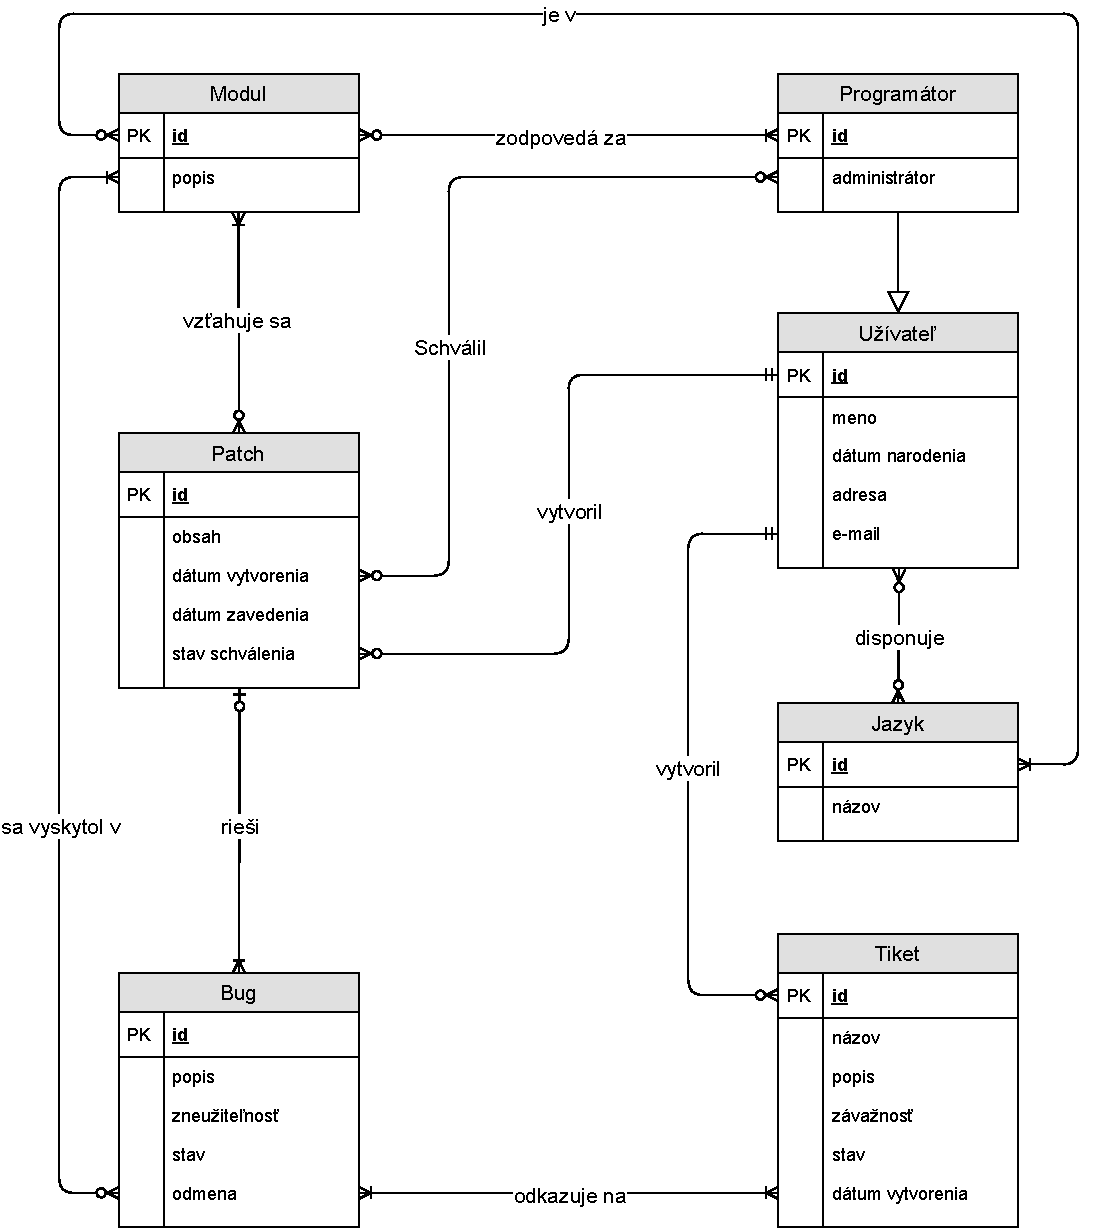
\includegraphics[width=0.95\linewidth]{ER_diagram.pdf}
        \vspace*{\fill}
    \end{center}

    \newpage

    \section{Popis výsledného skriptu}
    \label{sec:popis-výsledného-skriptu}

    \subsection{Drop existujúcich tabuliek}\label{subsec:drop-existujúcich-tabuliek}

    Pred vytvorením nových databázových objektov sa vykoná \texttt{DROP TABLE} pre každú vytvorenú tabuľku, \texttt{DROP SEQUENCE} pre sekvenciu a \texttt{DROP MATERIALIZED VIEW} pre materializovaný pohľad aby nedochádzalo k redefinícii už existujúcich tabuliek.
    Pri tabuľkách so závislosťami sa použije \texttt{CASCADE CONSTRAINTS} na odstránenie tabuľky a jej závislostí.

    \subsection{Vytvorenie nových tabuliek}\label{subsec:vytvorenie-nových-tabulieknull}

    Vytvoria sa tabuľky podľa špecifikácie ER diagramu zo sekcie~\ref{sec:entity-relationship-diagram}.
    Pre vzťahy many to many sa vytvorili nové pomocné tabuľky.
    Pre vzťahy one to many sa iba pridali codzie kľúče pomocou \texttt{ALTER TABLE} po vytvorení oboch tabuliek vzťahu.

    \subsection{Triggery\ -\ vytvorenie}\label{subsec:triggery}

    \begin{enumerate}
        \item \texttt{ticket\_id\_gen}
        Slúži na automatické generovanie hodnôt primárneho kľúča tabuľky \texttt{ticket} podľa sekvencie \texttt{ticket\_seq}.
        \item \texttt{patch\_created\_gen}
        Podobný trigger-u 1, generuje hodnotu aktuálneho času do stĺpca \texttt{created} tabuľky \texttt{patch}.
        \item \texttt{notify\_programmer}
        V prípade vytvorenia nového bugu notifikuje programátorov zodpovedných za modul v ktorom sa bug vyskytol.
        Notifikuje programátorov zodpovedných za modul ak je vytvorený nový bug.
    \end{enumerate}

    \subsection{Naplnenie databázy}\label{subsec:naplnenie-databázy}

    Po definovaní triggerov sa databáza naplní ukážkovými dátami (v tejto časti sql skriptu je aj ukážka použitia triggerov).

    \subsection{Triggery\ -\ použitie}\label{subsec:triggery---použitie}

    \begin{enumerate}
        \item \texttt{ticket\_id\_gen}
        Pred vykonaním INSERT-u do tabuľky \texttt{ticket} sa do stĺpca \texttt{id} vloží nasledujúca hodnota zo sekvencie.
        \item \texttt{patch\_created\_gen}
        Pred vykonaním INSERT-u do tabuľky \texttt{patch} sa do stĺpca \texttt{created} vygeneruje a vloží timestamp aktuálneho času.
        \item \texttt{notify\_programmer}
        Po vykonaní INSERT-u sa odošle notifikácia programátorom (v našom programe implementované iba ako \texttt{DBMS\_OUTPUT.PUT\_LINE()}).
    \end{enumerate}

    \subsection{Procedúry}\label{subsec:procedúry}

    \begin{enumerate}
        \item \texttt{p\_display\_ticket\_info}
        Zobrazí informácie o tickete (podľa id) a bugoch na ktoré odkazuje.
        Použije sa zavolaním \texttt{"p\_display\_ticket\_info"(ticket\_id);} kde \texttt{ticket\_id} je id ticketu na zobrazenie.

        \item \texttt{p\_display\_module\_info}
        Zobrazí informácie o module (podľa id), v akých jazykoch je implementovaný a kto zaň zodpovedá.
        Použije sa zavolaním \texttt{"p\_display\_module\_info"(module\_id);} kde \texttt{module\_id} je id modulu na zobrazenie.
    \end{enumerate}

    \subsection{Explain plan a index}\label{subsec:explain-plan-+-index}
%    TODO: add more content here

    Pre ukážku EXPLAIN PLAN sme si zvolili SELECT doposiaľ neschválených pachov ktoré sa týkajú viac ako jedného modulu (u týchto patchov je možné predpokladať záujem viacerých programátorov)
    Tento príkaz spojí 2 tabuľky, používa agregačnú funkciu \texttt{COUNT} a klauzulu \texttt{GROUP BY} podľa zadania.

    Pre zrýchlenie príkazu sme zaviedli nový index \texttt{index\_approved} na stĺpci \texttt{approved} tabuľky \texttt{patch}.

    \subsection{Prístupové práva}\label{subsec:prístupové-práva}

    Pre každú tabuľku a materializovaný pohľad je vykonaný príkaz \texttt{GRANT} s právami \texttt{ALL}.
    Pre procedúry postačí právo execute, preto je pre každú procedúru vykonaný príkaz \texttt{GRANT} s právom \texttt{EXECUTE}.

    \subsection{Materializovaný pohľad}\label{subsec:materializovaný-pohľad}

    Vytvorili sme materializovaný pohľad ktorý zobrazí všetky tickety, kto ich vytvoril a zoradí ich podľa statusu.
    Dáta v materializovanom pohľade sa neaktualizujú ak sa zmení hodnota v tabuľkách z ktorých je vytvorený.

\end{document}
